\documentclass[12pt,a4paper]{article}
\usepackage[utf8]{vietnam}
\usepackage{amsmath,amssymb}
\usepackage{tabularx}
\usepackage{tikz}
\usepackage{xcolor}
\usepackage[top=0.6cm, bottom=0.6cm, left=0.6cm, right=0.6cm]{geometry}
\usepackage[dethi]{ex_test}

\SAOPTN{widthSA=2.6,heightSA=0.62}
\setlength{\parskip}{0pt}

% Dong ke cham mo chuan viet tay
\newcommand{\dongke}[1]{%
  \begingroup%
  \setlength{\parskip}{0pt}%
  \baselineskip=18.5pt%
  \vspace{1.0mm}%
  \foreach \i in {1,...,#1}{%
    \noindent{\color{gray!60}\dotfill}\par%
  }%
  \vspace{0.6mm}%
  \endgroup%
}

% Dinh nghia o bai tap tu luan trong bang
\newcommand{\oBaiTap}[3][6]{%
  \vspace{1.0mm}%
  \noindent\textbf{#2} #3\par%
  \dongke{#1}%
}

\begin{document}
\pagestyle{empty}
% =============================================================================
% ========================= TOAN 9 TUAN 10 BUOI 02 - MA DE 101 =================
% ========================= TRANG 1/2 ==========================================
% =============================================================================
\noindent
\begin{tabularx}{\linewidth}{|X|c|}
\hline
\textbf{PHIẾU KIỂM TRA ĐỊNH KỲ TOÁN 9 - TUẦN 10 - BUỔI 2} & \textbf{Mã đề: 101 - Trang 1/2} \\
\hline
\end{tabularx}

\vspace{1.0mm}

\noindent
\begin{tabularx}{\linewidth}{|p{3.2cm}|X|}
\hline
\centering\textbf{ĐIỂM SỐ} & \centering\textbf{LỜI NHẬN XÉT CỦA THẦY CÔ} \tabularnewline
\hline
\rule{0pt}{1.8cm} & \tabularnewline
\hline
\end{tabularx}

\vspace{1.2mm}
\noindent\textbf{Câu 1 (0,25 điểm).} $MA, MB$ là tiếp tuyến của $(O)$ cắt nhau tại $M$. Khẳng định đúng là: \shortans{MA = MB}\par\vspace{0.5mm}
\noindent\textbf{Câu 2 (0,25 điểm).} $MA, MB$ là hai tiếp tuyến của $(O)$, biết $\widehat{AMB} = 60^\circ$. Số đo góc $\widehat{AOB}$ là: \shortans{120^\circ}\par\vspace{0.5mm}
\noindent\textbf{Câu 3 (0,25 điểm).} Tâm của đường tròn nội tiếp tam giác là giao điểm của ba đường: \shortans{\text{phân giác}}\par\vspace{0.5mm}
\noindent\textbf{Câu 4 (0,25 điểm).} Giá trị của biểu thức $\sqrt{(3 - \sqrt{10})^2}$ là: \shortans{\sqrt{10} - 3}\par\vspace{0.5mm}
\noindent\textbf{Câu 5 (0,25 điểm).} Điều kiện xác định của biểu thức $\dfrac{1}{\sqrt{x - 3}}$ là: \shortans{x > 3}\par\vspace{0.5mm}
\noindent\textbf{Câu 6 (0,25 điểm).} Nghiệm của phương trình $\sqrt{x} = 5$ là: \shortans{x = 25}\par\vspace{0.5mm}
\noindent\textbf{Câu 7 (0,25 điểm).} Hệ phương trình $\begin{cases} 3x - y = 5 \\ x + 2y = 4 \end{cases}$ có nghiệm $(x; y)$ là: \shortans{(2; 1)}\par\vspace{0.5mm}
\noindent\textbf{Câu 8 (0,25 điểm).} Cho đường tròn $(O; R = 5\text{ cm})$. Chu vi của đường tròn là: \shortans{10\pi\text{ cm}}\par\vspace{0.5mm}
\noindent\textbf{Câu 9 (0,25 điểm).} Một hình tròn có bán kính $R = 4\text{ cm}$. Diện tích của hình tròn là: \shortans{16\pi\text{ cm}^2}\par\vspace{0.5mm}
\noindent\textbf{Câu 10 (0,25 điểm).} Bánh xe đường kính $60\text{ cm}$ lăn quãng đường $180\pi\text{ cm}$ thì quay được: \shortans{3\text{ vòng}}\par\vspace{0.5mm}
\vspace{0.8mm}
\noindent\textbf{Câu 11 (2,5 điểm). Đại số tổng hợp:}
\vspace{0.6mm}

\noindent
\begin{tabularx}{\linewidth}{|X|X|}
\hline
\oBaiTap[19]{a) \quad (1,25 điểm)}{Giải hệ phương trình: $\begin{cases} 2(x + y) + 3(x - y) = 4 \\ (x + y) - 2(x - y) = 9 \end{cases}$} & 
\oBaiTap[19]{b) (1,25 điểm)}{Cho $Q = \dfrac{\sqrt{x} + 3}{\sqrt{x} + 1}$ ($x \ge 0$). Tìm các giá trị nguyên của $x$ để biểu thức $Q$ nhận giá trị nguyên.} \\
\hline
\end{tabularx}

\newpage
% =============================================================================
% ========================= TOAN 9 TUAN 10 BUOI 02 - MA DE 101 =================
% ========================= TRANG 2/2 ==========================================
% =============================================================================
\noindent
\begin{tabularx}{\linewidth}{|X|c|}
\hline
\textbf{TOÁN 9 - TUẦN 10 - BUỔI 2} & \textbf{Mã đề: 101 - Trang 2/2} \\
\hline
\end{tabularx}

\vspace{1.2mm}

\noindent
\begin{tabularx}{\linewidth}{|X|}
\hline
\vspace{0.5mm}
\textbf{Câu 12 (2,5 điểm).} Nhân dịp khai trương, một siêu thị điện máy giảm giá $10\%$ cho mặt hàng tivi và $15\%$ cho mặt hàng máy giặt theo giá niêm yết. Bác Nam mua một chiếc tivi và một chiếc máy giặt với tổng giá niêm yết là $20\text{ triệu đồng}$, nhưng nhờ chương trình giảm giá nên bác chỉ phải thanh toán số tiền là $17{,}4\text{ triệu đồng}$. Tính giá niêm yết của mỗi mặt hàng nêu trên.\par
\vspace{0.4mm}
\noindent\textit{Bài giải:}\dongke{15}
\\ \hline
\end{tabularx}

\vspace{1.2mm}

\noindent
\begin{tabularx}{\linewidth}{|X|}
\hline
\vspace{0.5mm}
\begin{minipage}[t]{0.68\linewidth}
\vspace{0pt}
\textbf{Câu 13 (2,5 điểm).} Cho đường tròn $(O; R)$ và điểm $M$ nằm bên ngoài đường tròn. Qua $M$ kẻ hai tiếp tuyến $MA, MB$ với đường tròn $(O)$ ($A, B$ là các tiếp điểm). Kẻ đường kính $BC$ của đường tròn $(O)$. Đoạn thẳng $OM$ cắt $AB$ tại $H$.\par\vspace{0.4mm}
\textbf{a) (1,25 điểm)} Chứng minh $OM \perp AB$ tại $H$. Cho $R = 15\text{ cm}, OM = 25\text{ cm}$, tính độ dài đoạn thẳng $AB$.\par\vspace{0.4mm}
\textbf{b) (1,25 điểm)} Chứng minh $AC \parallel OM$ và tính diện tích tam giác $MAB$.
\end{minipage}\hfill
\begin{minipage}[t]{0.30\linewidth}
\vspace{0pt}\centering
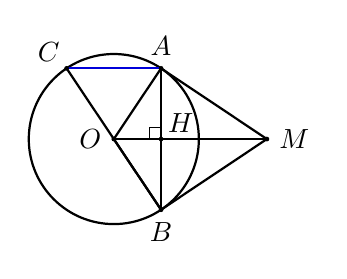
\begin{tikzpicture}[scale=0.72, >=stealth, line join=round, line cap=round]
  \coordinate (O) at (0, 0);
  \coordinate (M) at (2.7, 0);
  \coordinate (A) at (0.833, 1.247);
  \coordinate (B) at (0.833, -1.247);
  \coordinate (C) at (-0.833, 1.247);
  \coordinate (H) at (0.833, 0);
  
  \draw[thick] (O) circle (1.5);
  \draw[thick] (M) -- (A);
  \draw[thick] (M) -- (B);
  \draw[thick] (O) -- (M);
  \draw[thick] (O) -- (A);
  \draw[thick] (O) -- (B);
  \draw[thick] (A) -- (B);
  \draw[thick] (B) -- (C);
  \draw[thick, blue!85!black] (A) -- (C);
  
  % Right angle mark at H
  \draw (0.833, 0.2) -- (0.633, 0.2) -- (0.633, 0);
  
  \fill (O) circle (1.2pt) node[left=1pt] {$O$};
  \fill (M) circle (1.2pt) node[right=1pt] {$M$};
  \fill (A) circle (1.2pt) node[above=1pt] {$A$};
  \fill (B) circle (1.2pt) node[below=1pt] {$B$};
  \fill (C) circle (1.2pt) node[above left=-1pt] {$C$};
  \fill (H) circle (1.2pt) node[above right=-1pt] {$H$};
\end{tikzpicture}
\end{minipage}\par
\vspace{0.4mm}
\noindent\textit{Bài giải:}\dongke{15}
\\ \hline
\end{tabularx}

\newpage
% =============================================================================
% ========================= TOAN 9 TUAN 10 BUOI 02 - MA DE 102 =================
% ========================= TRANG 1/2 ==========================================
% =============================================================================
\noindent
\begin{tabularx}{\linewidth}{|X|c|}
\hline
\textbf{PHIẾU KIỂM TRA ĐỊNH KỲ TOÁN 9 - TUẦN 10 - BUỔI 2} & \textbf{Mã đề: 102 - Trang 1/2} \\
\hline
\end{tabularx}

\vspace{1.0mm}

\noindent
\begin{tabularx}{\linewidth}{|p{3.2cm}|X|}
\hline
\centering\textbf{ĐIỂM SỐ} & \centering\textbf{LỜI NHẬN XÉT CỦA THẦY CÔ} \tabularnewline
\hline
\rule{0pt}{1.8cm} & \tabularnewline
\hline
\end{tabularx}

\vspace{1.2mm}
\noindent\textbf{Câu 1 (0,25 điểm).} $MA, MB$ là hai tiếp tuyến của $(O)$ cắt nhau tại $M$. Tia $MO$ là phân giác của góc: \shortans{\widehat{AMB}}\par\vspace{0.5mm}
\noindent\textbf{Câu 2 (0,25 điểm).} $MA, MB$ là hai tiếp tuyến của $(O)$, biết $\widehat{AOB} = 110^\circ$. Số đo góc $\widehat{AMB}$ là: \shortans{70^\circ}\par\vspace{0.5mm}
\noindent\textbf{Câu 3 (0,25 điểm).} Tâm của đường tròn ngoại tiếp tam giác là giao điểm của ba đường: \shortans{\text{trung trực}}\par\vspace{0.5mm}
\noindent\textbf{Câu 4 (0,25 điểm).} Giá trị của biểu thức $\sqrt{(2 - \sqrt{5})^2}$ là: \shortans{\sqrt{5} - 2}\par\vspace{0.5mm}
\noindent\textbf{Câu 5 (0,25 điểm).} Điều kiện xác định của biểu thức $\dfrac{1}{\sqrt{x - 4}}$ là: \shortans{x > 4}\par\vspace{0.5mm}
\noindent\textbf{Câu 6 (0,25 điểm).} Nghiệm của phương trình $\sqrt{x} = 6$ là: \shortans{x = 36}\par\vspace{0.5mm}
\noindent\textbf{Câu 7 (0,25 điểm).} Hệ phương trình $\begin{cases} 3x - y = 7 \\ x + 2y = 7 \end{cases}$ có nghiệm $(x; y)$ là: \shortans{(3; 2)}\par\vspace{0.5mm}
\noindent\textbf{Câu 8 (0,25 điểm).} Cho đường tròn $(O; R = 6\text{ cm})$. Chu vi của đường tròn là: \shortans{12\pi\text{ cm}}\par\vspace{0.5mm}
\noindent\textbf{Câu 9 (0,25 điểm).} Một hình tròn có bán kính $R = 5\text{ cm}$. Diện tích của hình tròn là: \shortans{25\pi\text{ cm}^2}\par\vspace{0.5mm}
\noindent\textbf{Câu 10 (0,25 điểm).} Bánh xe đường kính $50\text{ cm}$ lăn quãng đường $200\pi\text{ cm}$ thì quay được: \shortans{4\text{ vòng}}\par\vspace{0.5mm}
\vspace{0.8mm}
\noindent\textbf{Câu 11 (2,5 điểm). Đại số tổng hợp:}
\vspace{0.6mm}

\noindent
\begin{tabularx}{\linewidth}{|X|X|}
\hline
\oBaiTap[19]{a) \quad (1,25 điểm)}{Giải hệ phương trình: $\begin{cases} 3(x + y) + 2(x - y) = 13 \\ 2(x + y) - (x - y) = 4 \end{cases}$} & 
\oBaiTap[19]{b) (1,25 điểm)}{Cho $Q = \dfrac{\sqrt{x} + 4}{\sqrt{x} + 1}$ ($x \ge 0$). Tìm các giá trị nguyên của $x$ để biểu thức $Q$ nhận giá trị nguyên.} \\
\hline
\end{tabularx}

\newpage
% =============================================================================
% ========================= TOAN 9 TUAN 10 BUOI 02 - MA DE 102 =================
% ========================= TRANG 2/2 ==========================================
% =============================================================================
\noindent
\begin{tabularx}{\linewidth}{|X|c|}
\hline
\textbf{TOÁN 9 - TUẦN 10 - BUỔI 2} & \textbf{Mã đề: 102 - Trang 2/2} \\
\hline
\end{tabularx}

\vspace{1.2mm}

\noindent
\begin{tabularx}{\linewidth}{|X|}
\hline
\vspace{0.5mm}
\textbf{Câu 12 (2,5 điểm).} Nhân dịp khai trương, một cửa hàng điện máy giảm giá $10\%$ cho mặt hàng tivi và $20\%$ cho mặt hàng máy giặt theo giá niêm yết. Bác Bình mua một chiếc tivi và một chiếc máy giặt với tổng giá niêm yết là $25\text{ triệu đồng}$, nhưng nhờ chương trình giảm giá nên bác chỉ phải thanh toán số tiền là $21{,}5\text{ triệu đồng}$. Tính giá niêm yết của mỗi mặt hàng nêu trên.\par
\vspace{0.4mm}
\noindent\textit{Bài giải:}\dongke{15}
\\ \hline
\end{tabularx}

\vspace{1.2mm}

\noindent
\begin{tabularx}{\linewidth}{|X|}
\hline
\vspace{0.5mm}
\begin{minipage}[t]{0.68\linewidth}
\vspace{0pt}
\textbf{Câu 13 (2,5 điểm).} Cho đường tròn $(O; R)$ và điểm $M$ nằm bên ngoài đường tròn. Qua $M$ kẻ hai tiếp tuyến $MA, MB$ với đường tròn $(O)$ ($A, B$ là các tiếp điểm). Kẻ đường kính $BC$ của đường tròn $(O)$. Đoạn thẳng $OM$ cắt $AB$ tại $H$.\par\vspace{0.4mm}
\textbf{a) (1,25 điểm)} Chứng minh $OM \perp AB$ tại $H$. Cho $R = 6\text{ cm}, OM = 10\text{ cm}$, tính độ dài đoạn thẳng $AB$.\par\vspace{0.4mm}
\textbf{b) (1,25 điểm)} Chứng minh $AC \parallel OM$ và tính diện tích tam giác $MAB$.
\end{minipage}\hfill
\begin{minipage}[t]{0.30\linewidth}
\vspace{0pt}\centering
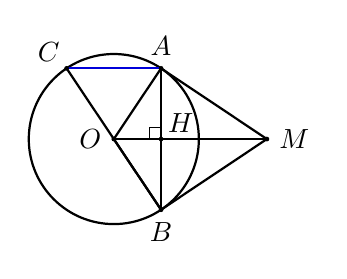
\begin{tikzpicture}[scale=0.72, >=stealth, line join=round, line cap=round]
  \coordinate (O) at (0, 0);
  \coordinate (M) at (2.7, 0);
  \coordinate (A) at (0.833, 1.247);
  \coordinate (B) at (0.833, -1.247);
  \coordinate (C) at (-0.833, 1.247);
  \coordinate (H) at (0.833, 0);
  
  \draw[thick] (O) circle (1.5);
  \draw[thick] (M) -- (A);
  \draw[thick] (M) -- (B);
  \draw[thick] (O) -- (M);
  \draw[thick] (O) -- (A);
  \draw[thick] (O) -- (B);
  \draw[thick] (A) -- (B);
  \draw[thick] (B) -- (C);
  \draw[thick, blue!85!black] (A) -- (C);
  
  % Right angle mark at H
  \draw (0.833, 0.2) -- (0.633, 0.2) -- (0.633, 0);
  
  \fill (O) circle (1.2pt) node[left=1pt] {$O$};
  \fill (M) circle (1.2pt) node[right=1pt] {$M$};
  \fill (A) circle (1.2pt) node[above=1pt] {$A$};
  \fill (B) circle (1.2pt) node[below=1pt] {$B$};
  \fill (C) circle (1.2pt) node[above left=-1pt] {$C$};
  \fill (H) circle (1.2pt) node[above right=-1pt] {$H$};
\end{tikzpicture}
\end{minipage}\par
\vspace{0.4mm}
\noindent\textit{Bài giải:}\dongke{15}
\\ \hline
\end{tabularx}

\newpage
% =============================================================================
% ========================= TOAN 9 TUAN 10 BUOI 02 - MA DE 103 =================
% ========================= TRANG 1/2 ==========================================
% =============================================================================
\noindent
\begin{tabularx}{\linewidth}{|X|c|}
\hline
\textbf{PHIẾU KIỂM TRA ĐỊNH KỲ TOÁN 9 - TUẦN 10 - BUỔI 2} & \textbf{Mã đề: 103 - Trang 1/2} \\
\hline
\end{tabularx}

\vspace{1.0mm}

\noindent
\begin{tabularx}{\linewidth}{|p{3.2cm}|X|}
\hline
\centering\textbf{ĐIỂM SỐ} & \centering\textbf{LỜI NHẬN XÉT CỦA THẦY CÔ} \tabularnewline
\hline
\rule{0pt}{1.8cm} & \tabularnewline
\hline
\end{tabularx}

\vspace{1.2mm}
\noindent\textbf{Câu 1 (0,25 điểm).} $MA, MB$ là hai tiếp tuyến của $(O)$ cắt nhau tại $M$. Tia $OM$ là phân giác của góc: \shortans{\widehat{AOB}}\par\vspace{0.5mm}
\noindent\textbf{Câu 2 (0,25 điểm).} $MA, MB$ là hai tiếp tuyến của $(O)$, biết $\widehat{AMB} = 80^\circ$. Số đo góc $\widehat{AOB}$ là: \shortans{100^\circ}\par\vspace{0.5mm}
\noindent\textbf{Câu 3 (0,25 điểm).} Tam giác vuông có hai cạnh góc vuông $6\text{ cm}$ và $8\text{ cm}$. Bán kính nội tiếp $r$ là: \shortans{2\text{ cm}}\par\vspace{0.5mm}
\noindent\textbf{Câu 4 (0,25 điểm).} Giá trị của biểu thức $\sqrt{(\sqrt{7} - 3)^2}$ là: \shortans{3 - \sqrt{7}}\par\vspace{0.5mm}
\noindent\textbf{Câu 5 (0,25 điểm).} Điều kiện xác định của biểu thức $\dfrac{1}{\sqrt{x - 5}}$ là: \shortans{x > 5}\par\vspace{0.5mm}
\noindent\textbf{Câu 6 (0,25 điểm).} Nghiệm của phương trình $\sqrt{x} = 7$ là: \shortans{x = 49}\par\vspace{0.5mm}
\noindent\textbf{Câu 7 (0,25 điểm).} Hệ phương trình $\begin{cases} 3x - y = 8 \\ x + 2y = 5 \end{cases}$ có nghiệm $(x; y)$ là: \shortans{(3; 1)}\par\vspace{0.5mm}
\noindent\textbf{Câu 8 (0,25 điểm).} Cho đường tròn $(O; R = 7\text{ cm})$. Chu vi của đường tròn là: \shortans{14\pi\text{ cm}}\par\vspace{0.5mm}
\noindent\textbf{Câu 9 (0,25 điểm).} Một hình tròn có bán kính $R = 3\text{ cm}$. Diện tích của hình tròn là: \shortans{9\pi\text{ cm}^2}\par\vspace{0.5mm}
\noindent\textbf{Câu 10 (0,25 điểm).} Bánh xe đường kính $70\text{ cm}$ lăn quãng đường $350\pi\text{ cm}$ thì quay được: \shortans{5\text{ vòng}}\par\vspace{0.5mm}
\vspace{0.8mm}
\noindent\textbf{Câu 11 (2,5 điểm). Đại số tổng hợp:}
\vspace{0.6mm}

\noindent
\begin{tabularx}{\linewidth}{|X|X|}
\hline
\oBaiTap[19]{a) \quad (1,25 điểm)}{Giải hệ phương trình: $\begin{cases} 4(x + y) + (x - y) = 11 \\ (x + y) - 3(x - y) = -7 \end{cases}$} & 
\oBaiTap[19]{b) (1,25 điểm)}{Cho $Q = \dfrac{\sqrt{x} + 5}{\sqrt{x} + 2}$ ($x \ge 0$). Tìm các giá trị nguyên của $x$ để biểu thức $Q$ nhận giá trị nguyên.} \\
\hline
\end{tabularx}

\newpage
% =============================================================================
% ========================= TOAN 9 TUAN 10 BUOI 02 - MA DE 103 =================
% ========================= TRANG 2/2 ==========================================
% =============================================================================
\noindent
\begin{tabularx}{\linewidth}{|X|c|}
\hline
\textbf{TOÁN 9 - TUẦN 10 - BUỔI 2} & \textbf{Mã đề: 103 - Trang 2/2} \\
\hline
\end{tabularx}

\vspace{1.2mm}

\noindent
\begin{tabularx}{\linewidth}{|X|}
\hline
\vspace{0.5mm}
\textbf{Câu 12 (2,5 điểm).} Nhân dịp lễ, một siêu thị điện máy giảm giá $20\%$ cho mặt hàng tivi và $15\%$ cho mặt hàng máy giặt theo giá niêm yết. Bác Cường mua một chiếc tivi và một chiếc máy giặt với tổng giá niêm yết là $30\text{ triệu đồng}$, nhưng nhờ chương trình giảm giá nên bác chỉ phải thanh toán số tiền là $24{,}6\text{ triệu đồng}$. Tính giá niêm yết của mỗi mặt hàng nêu trên.\par
\vspace{0.4mm}
\noindent\textit{Bài giải:}\dongke{15}
\\ \hline
\end{tabularx}

\vspace{1.2mm}

\noindent
\begin{tabularx}{\linewidth}{|X|}
\hline
\vspace{0.5mm}
\begin{minipage}[t]{0.68\linewidth}
\vspace{0pt}
\textbf{Câu 13 (2,5 điểm).} Cho đường tròn $(O; R)$ và điểm $M$ nằm bên ngoài đường tròn. Qua $M$ kẻ hai tiếp tuyến $MA, MB$ với đường tròn $(O)$ ($A, B$ là các tiếp điểm). Kẻ đường kính $BC$ của đường tròn $(O)$. Đoạn thẳng $OM$ cắt $AB$ tại $H$.\par\vspace{0.4mm}
\textbf{a) (1,25 điểm)} Chứng minh $OM \perp AB$ tại $H$. Cho $R = 9\text{ cm}, OM = 15\text{ cm}$, tính độ dài đoạn thẳng $AB$.\par\vspace{0.4mm}
\textbf{b) (1,25 điểm)} Chứng minh $AC \parallel OM$ và tính diện tích tam giác $MAB$.
\end{minipage}\hfill
\begin{minipage}[t]{0.30\linewidth}
\vspace{0pt}\centering
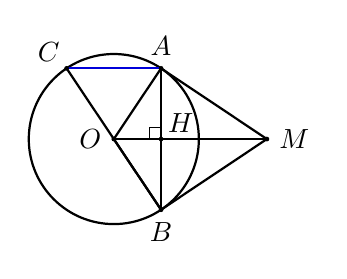
\begin{tikzpicture}[scale=0.72, >=stealth, line join=round, line cap=round]
  \coordinate (O) at (0, 0);
  \coordinate (M) at (2.7, 0);
  \coordinate (A) at (0.833, 1.247);
  \coordinate (B) at (0.833, -1.247);
  \coordinate (C) at (-0.833, 1.247);
  \coordinate (H) at (0.833, 0);
  
  \draw[thick] (O) circle (1.5);
  \draw[thick] (M) -- (A);
  \draw[thick] (M) -- (B);
  \draw[thick] (O) -- (M);
  \draw[thick] (O) -- (A);
  \draw[thick] (O) -- (B);
  \draw[thick] (A) -- (B);
  \draw[thick] (B) -- (C);
  \draw[thick, blue!85!black] (A) -- (C);
  
  % Right angle mark at H
  \draw (0.833, 0.2) -- (0.633, 0.2) -- (0.633, 0);
  
  \fill (O) circle (1.2pt) node[left=1pt] {$O$};
  \fill (M) circle (1.2pt) node[right=1pt] {$M$};
  \fill (A) circle (1.2pt) node[above=1pt] {$A$};
  \fill (B) circle (1.2pt) node[below=1pt] {$B$};
  \fill (C) circle (1.2pt) node[above left=-1pt] {$C$};
  \fill (H) circle (1.2pt) node[above right=-1pt] {$H$};
\end{tikzpicture}
\end{minipage}\par
\vspace{0.4mm}
\noindent\textit{Bài giải:}\dongke{15}
\\ \hline
\end{tabularx}

\newpage
% =============================================================================
% ========================= TOAN 9 TUAN 10 BUOI 02 - MA DE 104 =================
% ========================= TRANG 1/2 ==========================================
% =============================================================================
\noindent
\begin{tabularx}{\linewidth}{|X|c|}
\hline
\textbf{PHIẾU KIỂM TRA ĐỊNH KỲ TOÁN 9 - TUẦN 10 - BUỔI 2} & \textbf{Mã đề: 104 - Trang 1/2} \\
\hline
\end{tabularx}

\vspace{1.0mm}

\noindent
\begin{tabularx}{\linewidth}{|p{3.2cm}|X|}
\hline
\centering\textbf{ĐIỂM SỐ} & \centering\textbf{LỜI NHẬN XÉT CỦA THẦY CÔ} \tabularnewline
\hline
\rule{0pt}{1.8cm} & \tabularnewline
\hline
\end{tabularx}

\vspace{1.2mm}
\noindent\textbf{Câu 1 (0,25 điểm).} Hai tiếp tuyến tại $A, B$ của $(O)$ cắt nhau tại $M$. Đoạn $OM$ là đường trung trực của: \shortans{AB}\par\vspace{0.5mm}
\noindent\textbf{Câu 2 (0,25 điểm).} $MA, MB$ là hai tiếp tuyến của $(O)$, biết $\widehat{AOB} = 130^\circ$. Số đo góc $\widehat{AMB}$ là: \shortans{50^\circ}\par\vspace{0.5mm}
\noindent\textbf{Câu 3 (0,25 điểm).} Tam giác vuông có cạnh $5\text{ cm}, 12\text{ cm}, 13\text{ cm}$. Bán kính nội tiếp $r$ là: \shortans{2\text{ cm}}\par\vspace{0.5mm}
\noindent\textbf{Câu 4 (0,25 điểm).} Giá trị của biểu thức $\sqrt{(\sqrt{11} - 4)^2}$ là: \shortans{4 - \sqrt{11}}\par\vspace{0.5mm}
\noindent\textbf{Câu 5 (0,25 điểm).} Điều kiện xác định của biểu thức $\dfrac{1}{\sqrt{x - 2}}$ là: \shortans{x > 2}\par\vspace{0.5mm}
\noindent\textbf{Câu 6 (0,25 điểm).} Nghiệm của phương trình $\sqrt{x} = 8$ là: \shortans{x = 64}\par\vspace{0.5mm}
\noindent\textbf{Câu 7 (0,25 điểm).} Hệ phương trình $\begin{cases} 3x - y = 4 \\ x + 2y = 6 \end{cases}$ có nghiệm $(x; y)$ là: \shortans{(2; 2)}\par\vspace{0.5mm}
\noindent\textbf{Câu 8 (0,25 điểm).} Cho đường tròn $(O; R = 8\text{ cm})$. Chu vi của đường tròn là: \shortans{16\pi\text{ cm}}\par\vspace{0.5mm}
\noindent\textbf{Câu 9 (0,25 điểm).} Một hình tròn có bán kính $R = 6\text{ cm}$. Diện tích của hình tròn là: \shortans{36\pi\text{ cm}^2}\par\vspace{0.5mm}
\noindent\textbf{Câu 10 (0,25 điểm).} Bánh xe đường kính $40\text{ cm}$ lăn quãng đường $240\pi\text{ cm}$ thì quay được: \shortans{6\text{ vòng}}\par\vspace{0.5mm}
\vspace{0.8mm}
\noindent\textbf{Câu 11 (2,5 điểm). Đại số tổng hợp:}
\vspace{0.6mm}

\noindent
\begin{tabularx}{\linewidth}{|X|X|}
\hline
\oBaiTap[19]{a) \quad (1,25 điểm)}{Giải hệ phương trình: $\begin{cases} 2(x + y) + (x - y) = 7 \\ 3(x + y) - 2(x - y) = 7 \end{cases}$} & 
\oBaiTap[19]{b) (1,25 điểm)}{Cho $Q = \dfrac{\sqrt{x} + 7}{\sqrt{x} + 3}$ ($x \ge 0$). Tìm các giá trị nguyên của $x$ để biểu thức $Q$ nhận giá trị nguyên.} \\
\hline
\end{tabularx}

\newpage
% =============================================================================
% ========================= TOAN 9 TUAN 10 BUOI 02 - MA DE 104 =================
% ========================= TRANG 2/2 ==========================================
% =============================================================================
\noindent
\begin{tabularx}{\linewidth}{|X|c|}
\hline
\textbf{TOÁN 9 - TUẦN 10 - BUỔI 2} & \textbf{Mã đề: 104 - Trang 2/2} \\
\hline
\end{tabularx}

\vspace{1.2mm}

\noindent
\begin{tabularx}{\linewidth}{|X|}
\hline
\vspace{0.5mm}
\textbf{Câu 12 (2,5 điểm).} Nhân dịp tri ân khách hàng, một cửa hàng giảm giá $15\%$ cho mặt hàng tivi và $10\%$ cho mặt hàng máy giặt theo giá niêm yết. Bác Dũng mua một chiếc tivi và một chiếc máy giặt với tổng giá niêm yết là $18\text{ triệu đồng}$, nhưng nhờ chương trình giảm giá nên bác chỉ phải thanh toán số tiền là $15{,}7\text{ triệu đồng}$. Tính giá niêm yết của mỗi mặt hàng nêu trên.\par
\vspace{0.4mm}
\noindent\textit{Bài giải:}\dongke{15}
\\ \hline
\end{tabularx}

\vspace{1.2mm}

\noindent
\begin{tabularx}{\linewidth}{|X|}
\hline
\vspace{0.5mm}
\begin{minipage}[t]{0.68\linewidth}
\vspace{0pt}
\textbf{Câu 13 (2,5 điểm).} Cho đường tròn $(O; R)$ và điểm $M$ nằm bên ngoài đường tròn. Qua $M$ kẻ hai tiếp tuyến $MA, MB$ với đường tròn $(O)$ ($A, B$ là các tiếp điểm). Kẻ đường kính $BC$ của đường tròn $(O)$. Đoạn thẳng $OM$ cắt $AB$ tại $H$.\par\vspace{0.4mm}
\textbf{a) (1,25 điểm)} Chứng minh $OM \perp AB$ tại $H$. Cho $R = 12\text{ cm}, OM = 20\text{ cm}$, tính độ dài đoạn thẳng $AB$.\par\vspace{0.4mm}
\textbf{b) (1,25 điểm)} Chứng minh $AC \parallel OM$ và tính diện tích tam giác $MAB$.
\end{minipage}\hfill
\begin{minipage}[t]{0.30\linewidth}
\vspace{0pt}\centering
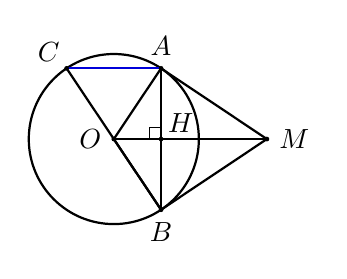
\begin{tikzpicture}[scale=0.72, >=stealth, line join=round, line cap=round]
  \coordinate (O) at (0, 0);
  \coordinate (M) at (2.7, 0);
  \coordinate (A) at (0.833, 1.247);
  \coordinate (B) at (0.833, -1.247);
  \coordinate (C) at (-0.833, 1.247);
  \coordinate (H) at (0.833, 0);
  
  \draw[thick] (O) circle (1.5);
  \draw[thick] (M) -- (A);
  \draw[thick] (M) -- (B);
  \draw[thick] (O) -- (M);
  \draw[thick] (O) -- (A);
  \draw[thick] (O) -- (B);
  \draw[thick] (A) -- (B);
  \draw[thick] (B) -- (C);
  \draw[thick, blue!85!black] (A) -- (C);
  
  % Right angle mark at H
  \draw (0.833, 0.2) -- (0.633, 0.2) -- (0.633, 0);
  
  \fill (O) circle (1.2pt) node[left=1pt] {$O$};
  \fill (M) circle (1.2pt) node[right=1pt] {$M$};
  \fill (A) circle (1.2pt) node[above=1pt] {$A$};
  \fill (B) circle (1.2pt) node[below=1pt] {$B$};
  \fill (C) circle (1.2pt) node[above left=-1pt] {$C$};
  \fill (H) circle (1.2pt) node[above right=-1pt] {$H$};
\end{tikzpicture}
\end{minipage}\par
\vspace{0.4mm}
\noindent\textit{Bài giải:}\dongke{15}
\\ \hline
\end{tabularx}
\end{document}
